%===============================================================================
\section{Application to Simulated Data}
\label{sec:app_on_sim_data}

We apply the hierarchical Bayesian model to estimate the model parameters of a simulated random sample of $100{,}000$ galaxies.
We compare the results of the Bayesian analysis to maximum likelihood and evaluate the performance of the GPU-based implementation.
The true values of the population parameters are listed in the first row of Tab.~\ref{tab:sum_est}.
The value of $\sigma_0$ in Eq.~\ref{eq:error} is chosen to be $\sigma_0=1$.
The flux limit is $T = 5.0$ and the distance limit is $r_{\max} \gtrsim 1.12 \times 10^{6}$.

We executed 1.5M burn-in and the same number of live MCMC steps to sample the probability distribution of the population parameters.
The length of the burn-in sequence was chosen by visual inspection of the autocorrelation plots.
To reduce autocorrelations in the Markov chain, $\theta$ samples were thinned and only every $150^\textnormal{th}$ sample was kept, hence the final number of samples was $10{,}000$.
Fig.~\ref{fig:results} shows the traces, histograms and autocorrelation plots of the population parameters whereas Tab.~\ref{tab:sum_est} lists the result in a numerical format.

\begin{table} \begin{center} \begin{tabular}{ l | d{12} | d{12} | d{12} | } \cline{2-4} & \beta & l & u \\ \hline \multicolumn{1}{|l|}{$\theta_\text{true}$} & -1.5 & 5.0\hphantom{000} \times 10^{10} & 5.0\hphantom{000} \times 10^{12} \\ \hline \multicolumn{1}{|l|}{$\theta_{\text{MCMC}}$} & -1.5037 & 5.0302 \times 10^{10} & 5.0000 \times 10^{12} \\ \hline \multicolumn{1}{|l|}{$\sigma_{\theta\text{,MCMC}}$} & 0.0059 & 3.3548 \times 10^{9} & 3.1806 \times 10^{10} \\ \hline \multicolumn{1}{|l|}{$\theta_{\text{MLE}}$} & -1.5564 & 7.3222 \times 10^{10} & 5.7207 \times 10^{12} \\ \hline \multicolumn{1}{|l|}{$\theta_{\text{MLE, no noise}}$} & -1.5009 & 4.9341 \times 10^{10} & 4.9819 \times 10^{12} \\ \hline \multicolumn{1}{|l|}{$\lvert \theta_{\text{true}} - \theta_{\text{MLE}} \rvert$} & >9.5525 \cdot \sigma_{\beta\text{,MCMC}} & >6.9221\cdot\sigma_{l\text{,MCMC}} & >22.6591\cdot\sigma_{u\text{,MCMC}} \\ \hline \end{tabular} \end{center} \caption{Summary of parameter estimation results.
The first row of the table indicates the true values which the simulated data was generated with.
The second row shows the mean of the distributions coming of the Bayesian model, whereas the third row contains the standard deviation of them.
For reference, we indicate the outcome of the ML estimatior run on the simulated data with and without noise in rows 4~and~5, respectively.
To compare the Bayesian model to ML, the last row of the table shows the difference between the ML estimator and the true values in terms of the standard deviation of the posterior from the Bayesian model.} \label{tab:sum_est} \end{table}

\begin{figure}
    \centering
    \begin{subfigure}{0.3\textwidth}
        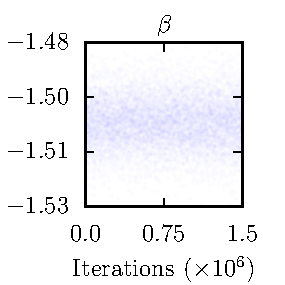
\includegraphics{{fig/beta}}
    \end{subfigure}
    \begin{subfigure}{0.3\textwidth}
        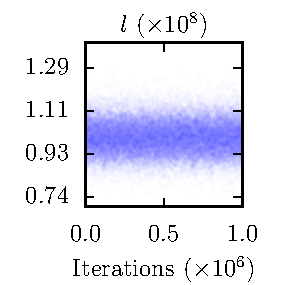
\includegraphics{{fig/lowerscale}}
    \end{subfigure}
    \begin{subfigure}{0.3\textwidth}
        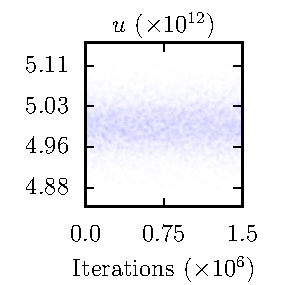
\includegraphics{{fig/upperscale}}
    \end{subfigure}
    
    \begin{subfigure}{0.3\textwidth}
        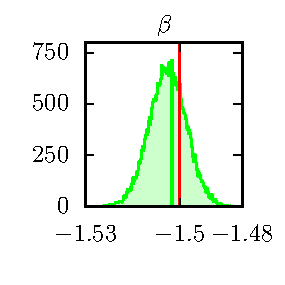
\includegraphics{{fig/beta_histo}}
    \end{subfigure}
    \begin{subfigure}{0.3\textwidth}
        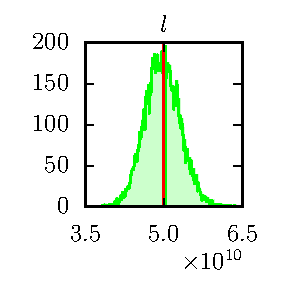
\includegraphics{{fig/lowerscale_histo}}
    \end{subfigure}
    \begin{subfigure}{0.3\textwidth}
        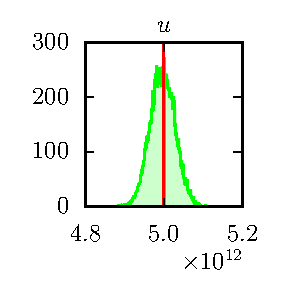
\includegraphics{{fig/upperscale_histo}}
    \end{subfigure}    
    
    \begin{subfigure}{0.3\textwidth}
        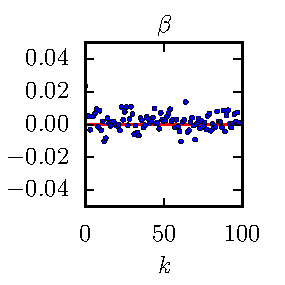
\includegraphics{{fig/autocorr_beta}}
    \end{subfigure}
    \begin{subfigure}{0.3\textwidth}
        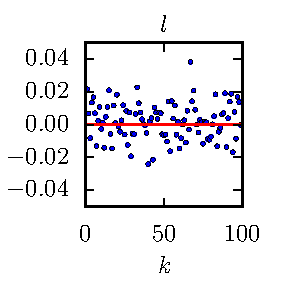
\includegraphics{{fig/autocorr_lowerscale}}
    \end{subfigure}
    \begin{subfigure}{0.3\textwidth}
        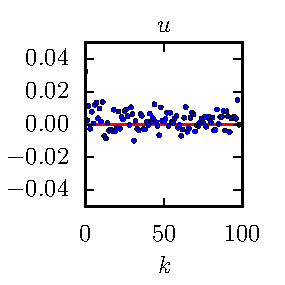
\includegraphics{{fig/autocorr_upperscale}}
    \end{subfigure}    
    \caption{Trace (upper row), histogram (middle row) and autocorrelation (lower row) plots of the three population parameters. The red vertical line overplotted the histograms show the true value of the parameter. With the exception of $\beta$, Bayesian modelling can recover model parameters with excellent accuracy.}
	\label{fig:results}
\end{figure}

%-------------------------------------------------------------------------------
\subsection{Performance tests}

\begin{figure}
   	\begin{center}
   		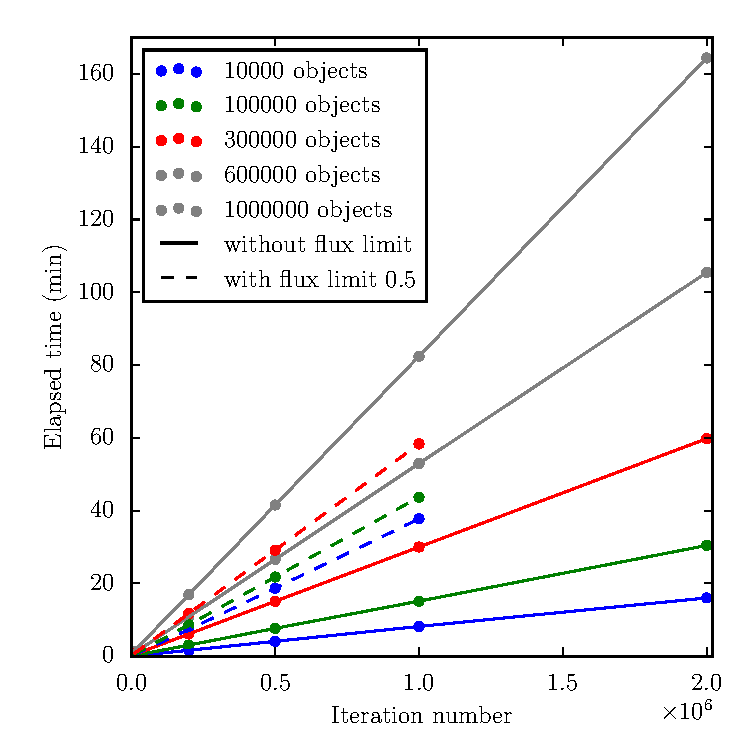
\includegraphics{{fig/performance_iter_vs_time}}
   	\end{center} 
    \caption{Runtime of the GPU code as a function of iterations for different numbers of objects, with (solid lines) and without (dashed lines) considering a flux limit of $T = 0.5$. Taking the flux limit into account results in an approximately fourfold increase of runtime.}
    \label{fig:performance_iter_vs_time}
\end{figure}

\begin{figure}
   	\begin{center}
   		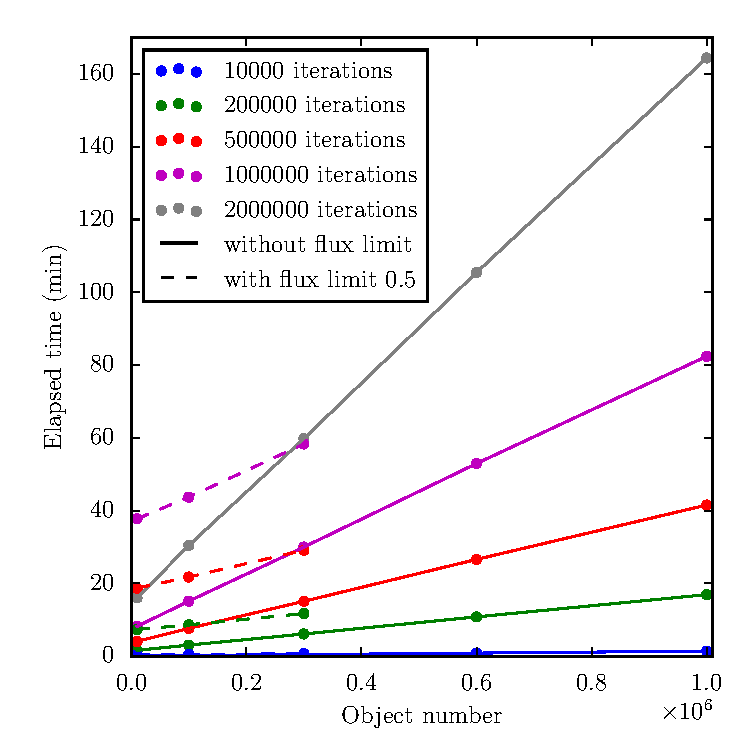
\includegraphics{{fig/performance_obj_vs_time}}
   	\end{center} 
    \caption{Runtime of the GPU code as a function of the number of objects, after a given number of iterations, with (solid lines) and without (dashed lines) considering a flux limit of $T = 0.5$. Taking the flux limit into account results in an approximately fourfold increase of runtime. On the other hand, the scaling of runtime with the number of objects is linear. This is due to the fact that fluxes are statistical independence, hence their distribution can be sampled in parallel on the GPU.}
    \label{fig:performance_obj_vs_time}
\end{figure}

We used NVIDIA Tesla K40c cards for the performance tests.
First, we executed tests without imposing a flux limit, which is a much simpler case as it does not contain the time-consuming numerical integration of Eq.~\ref{eq:mu}.
Next, we executed the with the flux limit turned on.
Fig.~\ref{fig:performance_iter_vs_time} shows the elapsed time as a function of iteration number (non-thinned) for different number of objects.
The functions are trivially linear as iteration steps always take a fixed amount of time.
More informative is Fig.~\ref{fig:performance_obj_vs_time} where we plot the elapsed time as a function of the number of objects for various numbers of iteration steps.
The linear scaling of computation time with the number of objects is due to the fact that the characteristics are independent.
As it is visible from the figures, turning on the flux limit clearly decreases the performance.
Real galaxy catalogs contain objects on the order of $10^8$, two magnitudes more than our simulated data set.
Extrapolating from out performance numbers, estimating the parameters of the luminosity function with $2 \times 10^5$ Markov steps would take about 2000 minutes, a bit less then one and a half days, which makes applying our method to real data feasible.

